\documentclass{article}

\usepackage{graphicx}
\usepackage{tikz}
\usepackage{tikzsymbols}
\usetikzlibrary{calc,patterns,shapes.geometric}
\pagestyle{empty}
\usepackage[margin=0pt]{geometry}
\geometry{papersize={14in,12in}}

\def\centerarc[#1](#2)(#3:#4:#5){\draw[#1] ($(#2)+({#5*cos(#3)},{#5*sin(#3)})$) arc (#3:#4:#5);}

\begin{document}
	\begin{figure}
		\centering
		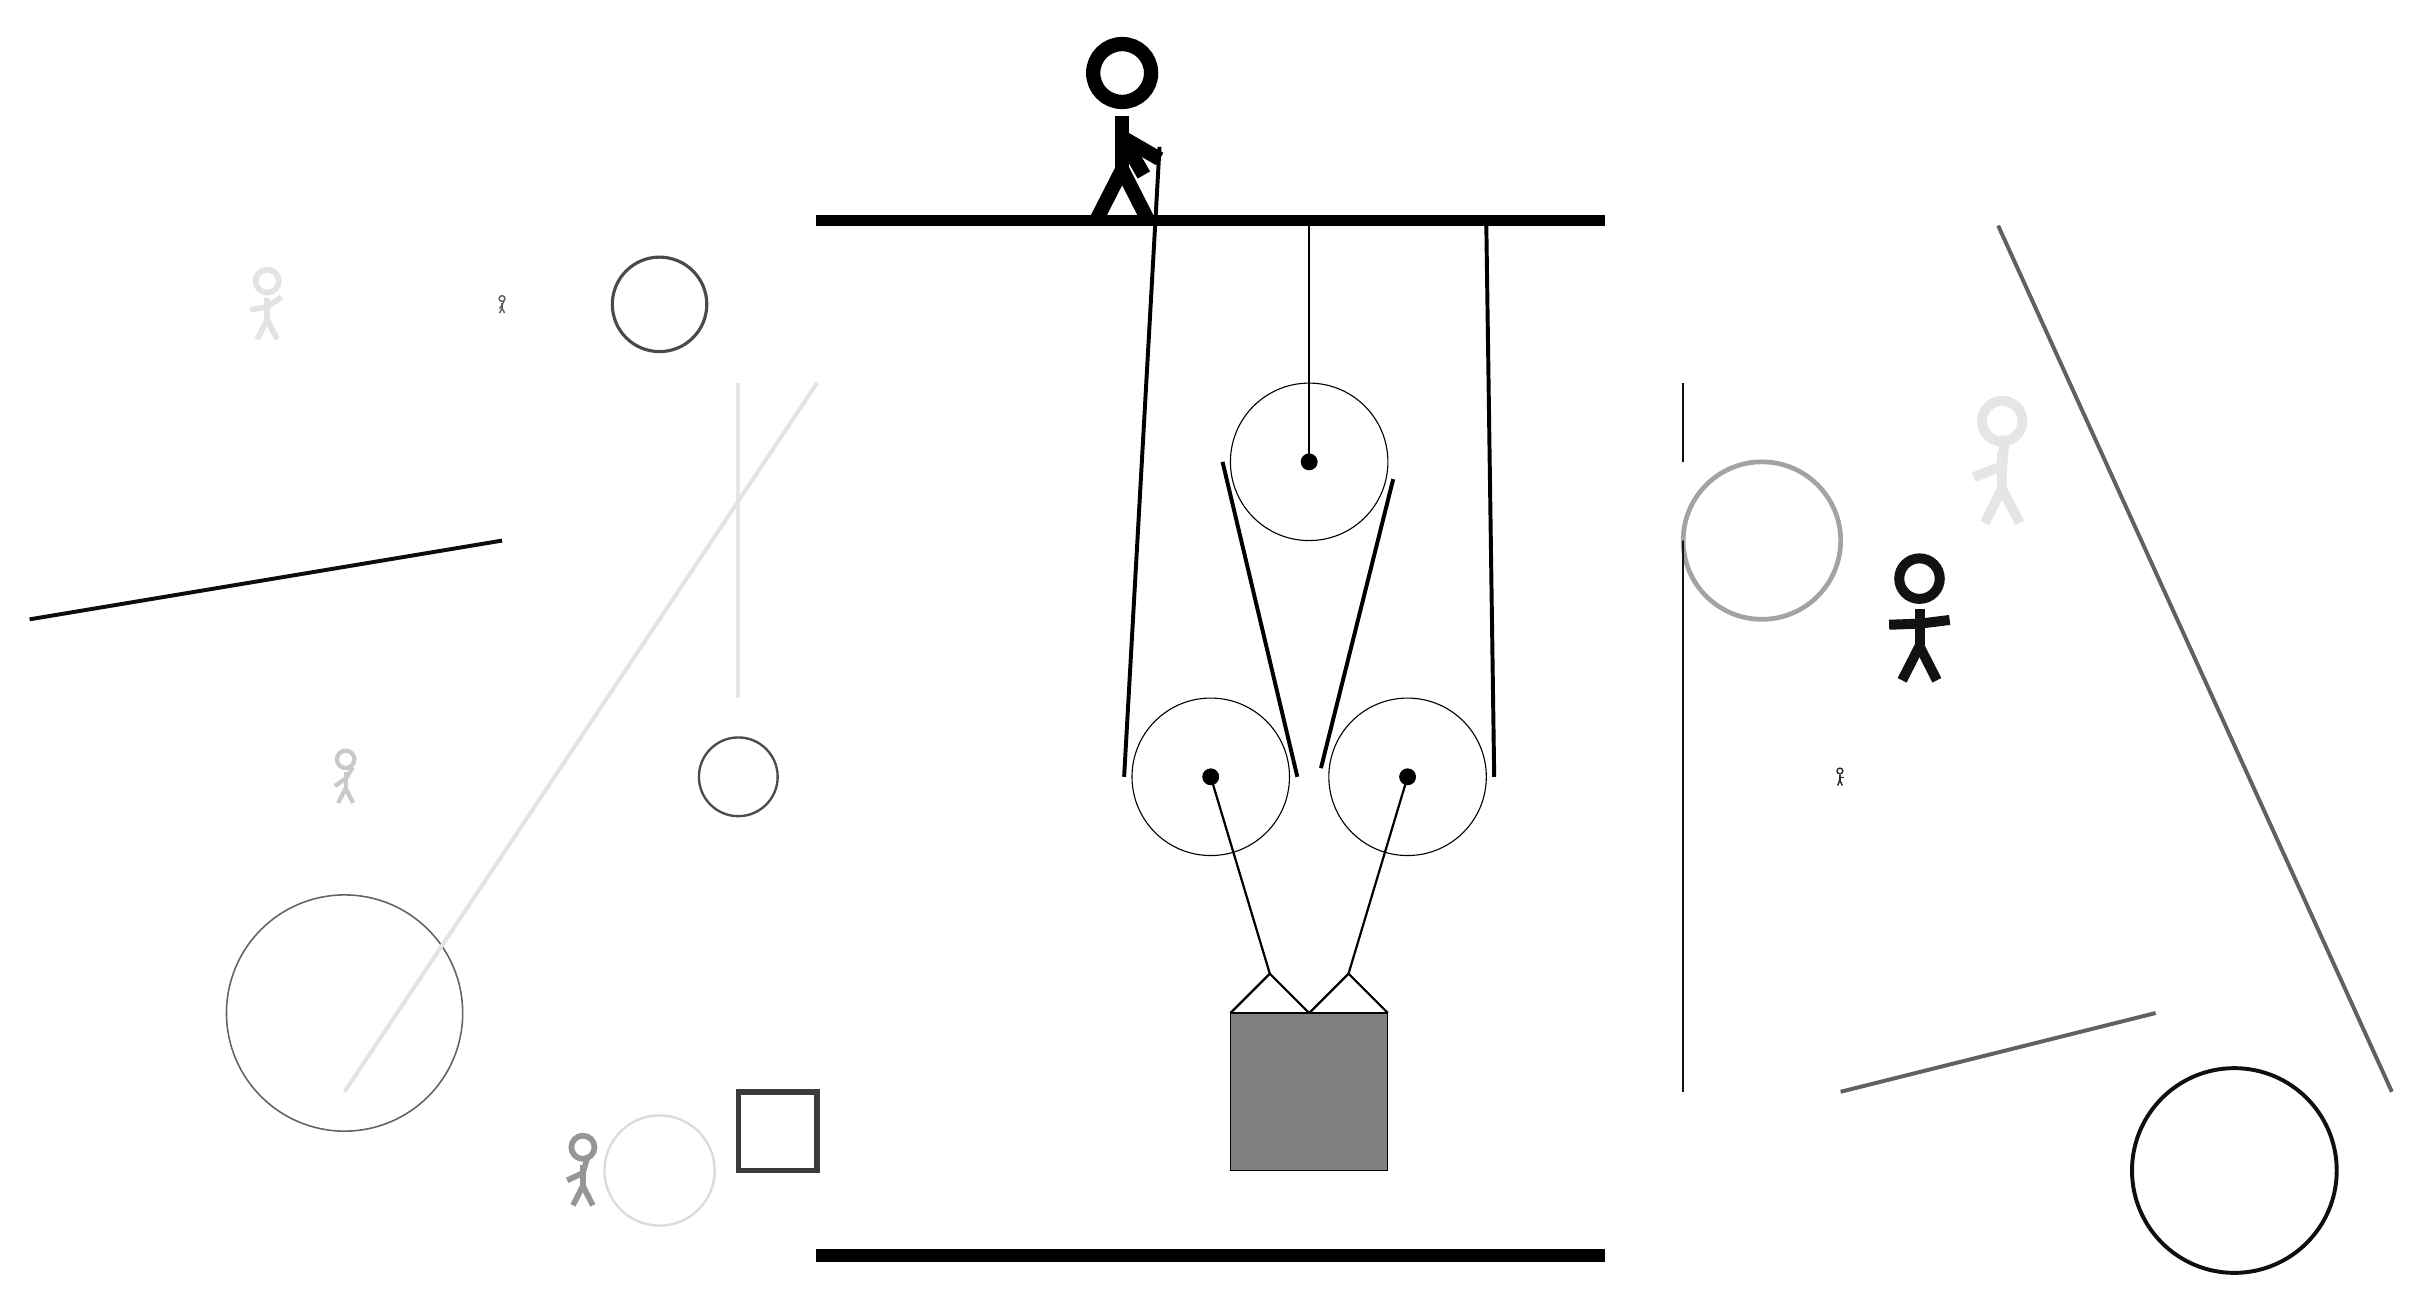
\begin{tikzpicture}
			%%%%% START %%%%%
			
			\draw[fill=black] (-4, 10) rectangle (6, 10.125);
			
			\node[line width=0.3mm, color=black!10] at (11, 7) {\Strichmaxerl[7][21][85]};
			
			\node[line width=0.4mm, color=black!62] at (-8, 9) {\Strichmaxerl[1][55][64]};
			\draw[line width=0.5mm, color=black!62](9, -1) -- (13, 0);
			\draw[line width=0.5mm, color=black!10](-5, 8) -- (-5, 4);
			\node[line width=0.4mm, color=black!41] at (-7, -2) {\Strichmaxerl[4][25][74]};
			\draw [line width=0.6mm, color=black!36](8, 6) circle (1.0);
			
			\draw [line width=0.5mm, color=black!94](14, -2) circle (1.3);
			
			\draw [line width=0.2mm, color=black!61](-10, 0) circle (1.5);
			\draw [line width=0.3mm, color=black!70](-5, 3) circle (0.5);
			
			\draw[line width=0.5mm, color=black!95](-8, 6) -- (-14, 5);
			
			\node[line width=0.5mm, color=black!11] at (-11, 9) {\Strichmaxerl[4][10][34]};
			\node[line width=0.5mm, color=black!83] at (9, 3) {\Strichmaxerl[1][80][0]};
			\draw [line width=0.3mm, color=black!14](-6, -2) circle (0.7);
			
			\draw[line width=0.3mm, color=black!92] (7, 6) rectangle (7, -1);
			\node[line width=0.2mm, color=black!93] at (10, 5) {\Strichmaxerl[7][2][7]};
			\draw [line width=0.4mm, color=black!71](-6, 9) circle (0.6);
			\draw[line width=0.3mm, color=black!94] (7, 7) rectangle (7, 8);
			\draw[line width=0.5mm, color=black!11](-4, 8) -- (-10, -1);
			\draw[line width=0.7mm, color=black!77] (-4, -2) rectangle (-5, -1);
			\node[line width=0.3mm, color=black!21] at (-10, 3) {\Strichmaxerl[3][34][57]};
			\draw[line width=0.5mm, color=black!62](11, 10) -- (16, -1);
			
			
			\draw (1, 3.0) circle (1);
			\draw[fill=black] (1, 3.0) circle (0.1);
			
			\draw (2.25, 7.0) circle (1);
			\draw[fill=black] (2.25, 7.0) circle (0.1);
			\draw[thick] (2.25, 7.0) -- (2.25, 10);
			
			\draw (3.5, 3.0) circle (1);
			\draw[fill=black] (3.5, 3.0) circle (0.1);
			
			\draw[thick] (3.5, 3.0) -- (2.75, 0.5);
			\draw[thick] (1, 3.0) -- (1.75, 0.5);
			\draw[thick]  (1.25, 0) -- (1.75, 0.5) -- (2.25, 0);
			\draw[thick]  (2.25, 0) -- (2.75, 0.5) -- (3.25, 0);
			\draw[fill=black!50] (1.25, 0) rectangle (3.25, -2);
			
			\draw[line width=0.5mm] (0.35, 11) --  (-0.1, 3.0);
			\centerarc[line width=0.5mm](1, 3.0)(180:360:1.1);
			\draw[line width=0.5mm] (2.1, 3.0) -- (1.15, 7.0);
			\centerarc[line width=0.5mm](2.25, 7.0)(-20:180:1.1);
			\draw[line width=0.5mm](3.317, 6.78) -- (2.4, 3.11);
			\centerarc[line width=0.5mm](3.5, 3.0)(160:360:1.1);
			\draw[line width=0.5mm](4.6, 3.0) -- (4.5, 10);
			
			\node at (-0.07, 11.2) {\Strichmaxerl[10][120][-30]};
			
			\draw[fill=black] (-4, -3) rectangle (6, -3.15);
			
			%%%%% END %%%%%
		\end{tikzpicture}
	\end{figure}	
\end{document}